
%(BEGIN_QUESTION)
% Copyright 2011, Tony R. Kuphaldt, released under the Creative Commons Attribution License (v 1.0)
% This means you may do almost anything with this work of mine, so long as you give me proper credit

A student wishes to build a resistor network useful for simulating a 100 ohm platinum RTD with an alpha value of 0.00392 $\Omega$/$\Omega$/$^{o}$C, over a temperature range of 0 degrees C to 200 degrees C.  The student's intent is to calculate the exact fixed-resistor values necessary to limit the potentiometer's range to the values corresponding to 0 and 200 degrees C:

$$\includegraphics[width=15.5cm]{i03436x01.eps}$$

$R_1$ = \underbar{\hskip 50pt} ohms

\vskip 10pt

$R_2$ = \underbar{\hskip 50pt} ohms

\vskip 10pt

Also, determine whether the simulated RTD temperature will {\it increase} or {\it decrease} as the potentiometer's shaft is turned clockwise.

\vskip 10pt

\underbar{file i03436}
%(END_QUESTION)





%(BEGIN_ANSWER)

$R_1$ = \underbar{\bf 100} ohms

\vskip 10pt

$R_2$ = \underbar{\bf 85.069} ohms

\vskip 10pt

The simulated RTD temperature will {\bf increase} as the potentiometer's shaft is turned clockwise.

\vskip 10pt

4 points for each correct resistor value, 2 points for proper direction of simulated temperature change.

%(END_ANSWER)





%(BEGIN_NOTES)

{\bf This question is intended for exams only and not worksheets!}.

%(END_NOTES)

